% Section: Generative AI for Synthetic Data Augmentation
% Source: 04_synthetic_data_augmentation.ipynb
%
% Required packages (load in the main document preamble):
%   \usepackage{graphicx}
%   \usepackage{amsmath}
%   \usepackage{booktabs}
%   \usepackage{hyperref}
%
% Figures referenced below live in figures/ next to this file; add that
% directory to the graphics path in the main document if needed:
%   \graphicspath{{latex/figures/}}

\section{Generative AI for Synthetic Data Augmentation}
\label{sec:synthetic-augmentation}

This section builds a pipeline for \textbf{synthetic bone marrow smear images} to
augment the plasma cell detection training set. A generative model is trained on
real plasma cells and the generated cells are composed onto synthetic background
templates to form full smears. The pipeline covers:

\begin{enumerate}
    \item Estimating a slide's background light and other per-slide statistics.
    \item Modeling those statistics with Kernel Density Estimation (KDE) to
          generate synthetic background templates.
    \item Cropping plasma cells from bone marrow smear images and isolating each
          one with its segmentation mask.
    \item Transforming crops into a new color space (color deconvolution), using
          each slide's background light.
    \item Training a generative (diffusion) model on those maps to synthesize new
          cells.
    \item Composing the generated synthetic cells onto templates to create new
          synthetic smear images.
    \item Checking whether this synthetic augmentation improves a detector on
          held-out test data.
\end{enumerate}

\subsection{Per-Slide Statistics}
\label{subsec:per-slide-statistics}

A \textbf{background template} is a synthetic slide layout (a background color
plus cell positions and sizes) sampled to match real slides statistically without
copying any. Section~\ref{subsec:kde-templates} fits KDE models over per-slide
statistics to generate these templates; generated cells
(Sections~\ref{subsec:crop-mask}--\ref{subsec:generate-cells}) are pasted onto the
sampled positions (Section~\ref{subsec:compose-smears}). Each real slide is
characterized by:

\begin{itemize}
    \item \textbf{Background light} --- the slide's background color, used later
          to normalize the color space.
    \item \textbf{Cell count, size and position} --- how many plasma cells, and
          their layout.
\end{itemize}

\subsubsection{Background Light Estimation}

Each slide has its own background light (the color of its unstained regions),
which varies with staining intensity and illumination at the time of capture. It
is estimated by downsampling the slide to a thumbnail, clustering its pixel
colors with K-Means ($k=5$), and picking the \textbf{brightest centroid}, since
background pixels are assumed to be brighter than cells and debris.
Figure~\ref{fig:bg-light} demonstrates this on three sample slides with visibly
different background colors.

\begin{figure}[htbp]
    \centering
    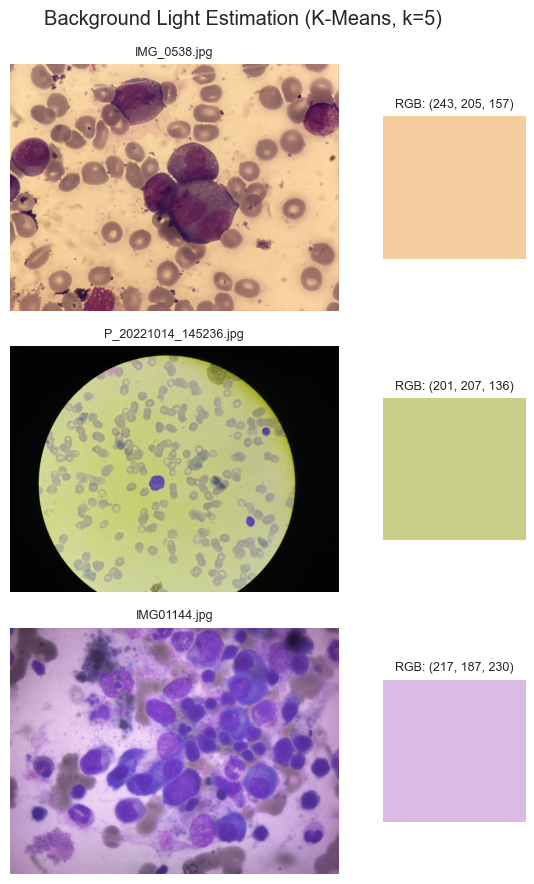
\includegraphics[width=0.55\textwidth]{figures/cell10.png}
    \caption{Background light estimation via K-Means ($k=5$) on three sample
    slides. The brightest cluster centroid (right swatches) is taken as each
    slide's background color.}
    \label{fig:bg-light}
\end{figure}

\subsubsection{Cell Count, Size and Position}

Besides the background light, a slide is characterized by its plasma cells: how
many, and each one's position and size. This comes from the YOLO label file
shipped with every image --- one box per line, \texttt{class\_id x\_center
y\_center width height}, with the four box coordinates normalized to $[0,1]$.
Only class \texttt{0} (\texttt{plasma\_cell}) boxes are kept. Since slides have
different aspect ratios, each image is first padded to a square (centered on the
shorter side) so that a given $x$ or $w$ means the same position/size on any
slide. Figure~\ref{fig:cell-boxes} shows the recovered boxes drawn back onto the
three sample slides.

\begin{figure}[htbp]
    \centering
    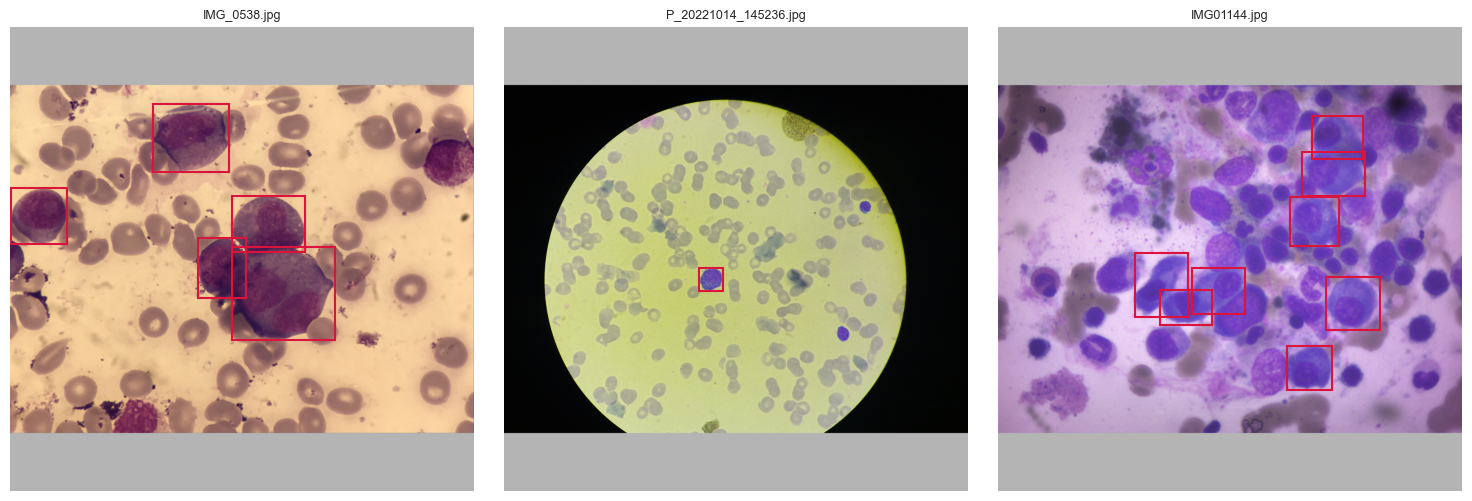
\includegraphics[width=\textwidth]{figures/cell13.png}
    \caption{Plasma cell bounding boxes (class \texttt{0}) recovered from the
    YOLO label files and drawn back onto the padded sample slides.}
    \label{fig:cell-boxes}
\end{figure}

The same statistics are precomputed for all 512 training slides and saved as two
tables: \texttt{slides.csv} (one row per slide: background light, plasma cell
count, image dimensions) and \texttt{cell\_boxes.csv} (one row per plasma cell:
position and size on the padded square).

\subsection{Modeling the Statistics with KDE}
\label{subsec:kde-templates}

A Kernel Density Estimate (KDE) fits a smooth density to a set of observations;
sampling from it gives new values with the same distribution as the real data,
without copying any slide. One KDE is fit per quantity that defines a template:

\begin{itemize}
    \item \textbf{counts} --- plasma cells per slide;
    \item \textbf{background} --- background light color, jointly over R, G, B;
    \item \textbf{coords} --- cell position on the square, jointly over $(x, y)$;
    \item \textbf{sizes} --- cell scale, taken as $\max(w, h)$.
\end{itemize}

Each quantity is bounded (counts $\geq 1$, colors in $[0,255]$, coordinates and
sizes in $[0,1]$), so each KDE is wrapped in a helper that rejects out-of-bounds
samples. A template is then generated by drawing a background color, a cell
count, and that many positions and sizes, placing boxes one at a time and
skipping any that would overlap one already placed. Figure~\ref{fig:templates}
shows three sampled templates.

\begin{figure}[htbp]
    \centering
    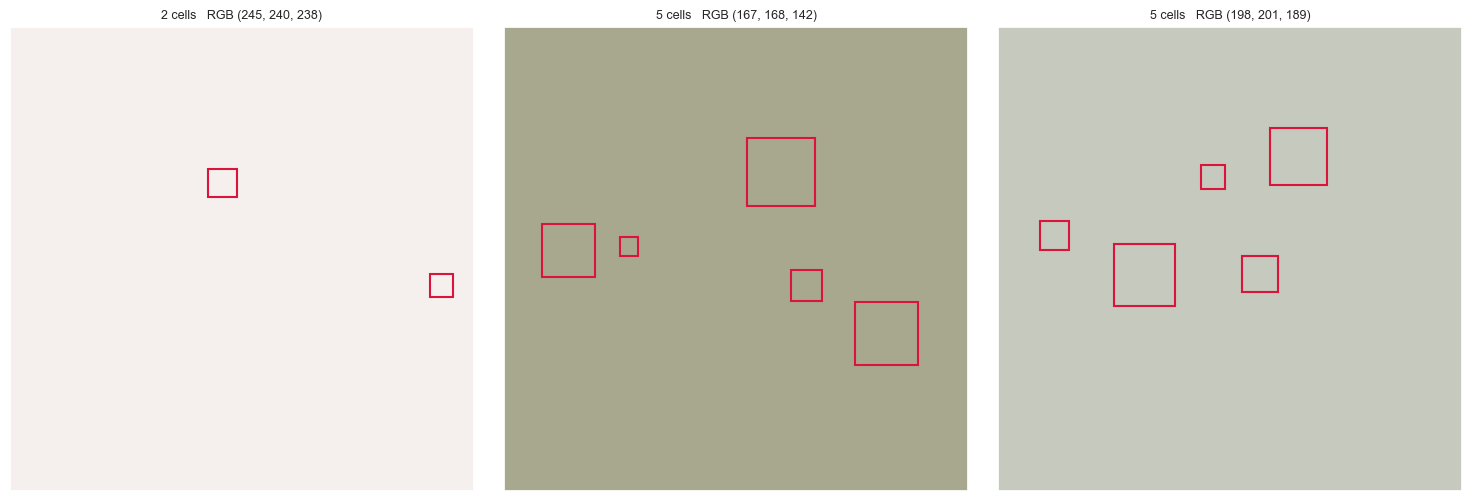
\includegraphics[width=\textwidth]{figures/cell19.png}
    \caption{Synthetic background templates sampled from the fitted KDEs: a
    background color plus non-overlapping cell positions and sizes.}
    \label{fig:templates}
\end{figure}

\subsection{Cropping and Masking the Plasma Cells}
\label{subsec:crop-mask}

A plasma cell \textbf{crop} is the patch of slide pixels inside one of the
bounding boxes from Section~\ref{subsec:per-slide-statistics}.
Figure~\ref{fig:crop-demo} demonstrates this on a single box from a sample
slide, cropping from the padded square so the coordinates match those computed
earlier.

\begin{figure}[htbp]
    \centering
    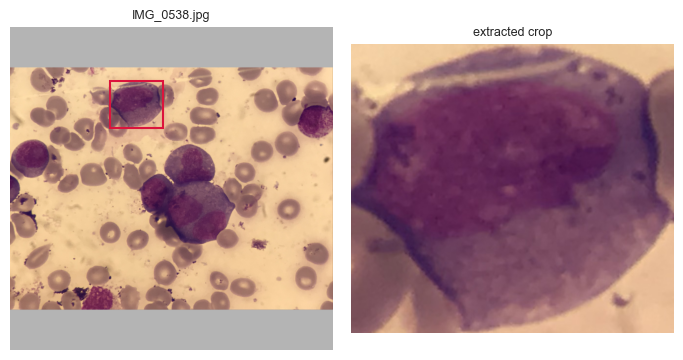
\includegraphics[width=0.65\textwidth]{figures/cell21.png}
    \caption{Extracting a single plasma-cell crop from its source slide.}
    \label{fig:crop-demo}
\end{figure}

The full set of crops is precomputed, one per cell, together with a binary
segmentation mask of the same name (255 on the cell, 0 on the background).
Figure~\ref{fig:crops-masks} shows, for every cell on one slide: the crop, its
mask, and the crop with the background removed via the mask. This masked cell
is the input to the color deconvolution step
(Section~\ref{subsec:color-deconvolution}).

\begin{figure}[htbp]
    \centering
    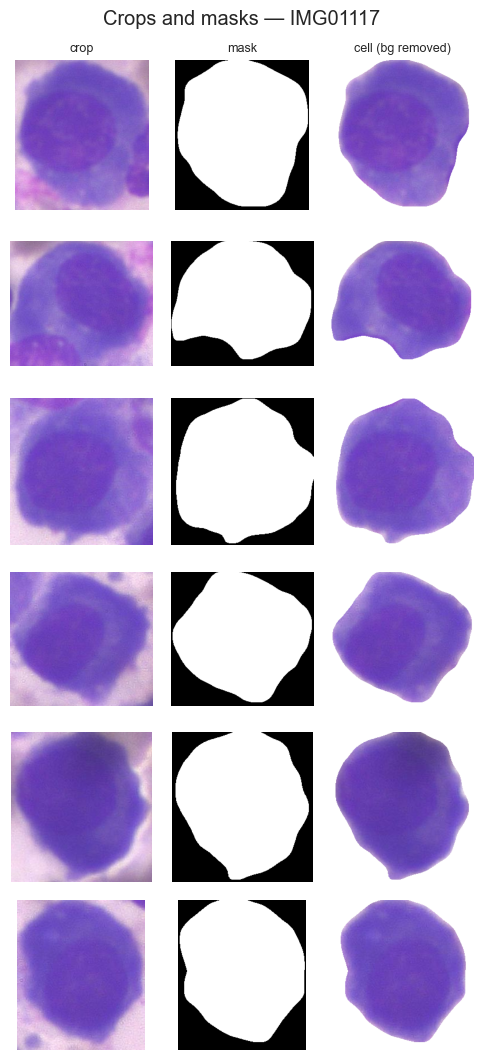
\includegraphics[width=0.4\textwidth]{figures/cell24.png}
    \caption{Crops, segmentation masks, and background-removed cells for every
    plasma cell on one sample slide.}
    \label{fig:crops-masks}
\end{figure}

\subsection{Color Deconvolution}
\label{subsec:color-deconvolution}

Stained cells are represented by dye concentration instead of raw RGB. Under
transmitted light, the Beer-Lambert law makes \textbf{optical density} linear in
dye concentration:

\begin{equation}
    \text{OD} = -\log_{10}\!\left(\frac{I}{I_0}\right)
    \label{eq:beer-lambert}
\end{equation}

where $I$ is the pixel color and $I_0$ the background light (the per-slide value
from Section~\ref{subsec:per-slide-statistics}). Each dye is a unit RGB
absorption vector; stacking the two Wright-Giemsa dyes (\textbf{Azure~B} and
\textbf{Eosin~Y}) gives a $2\times3$ \textbf{stain matrix} $S$. Since
$\text{OD} = C \cdot S$, the two concentrations $C$ are obtained as
$\text{OD} \cdot S^{+}$ (least-squares via the pseudo-inverse), clipped at zero
--- mapping each 3-channel crop to a \textbf{2-channel concentration map}.
Figure~\ref{fig:deconvolution} shows the result for the masked cells of
Figure~\ref{fig:crops-masks}, using each cell's source-slide background light as
$I_0$.

\begin{figure}[htbp]
    \centering
    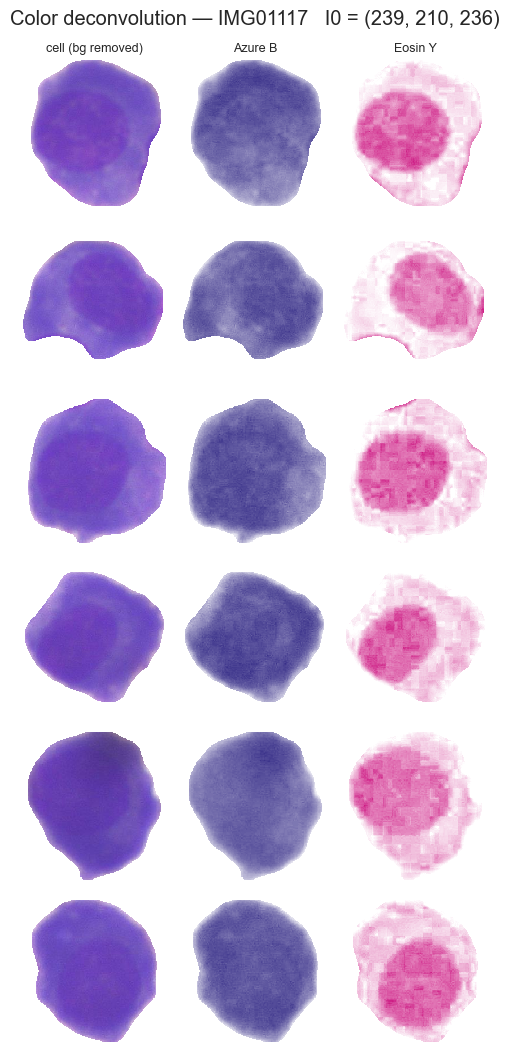
\includegraphics[width=0.4\textwidth]{figures/cell27.png}
    \caption{Color deconvolution of the masked cells into per-dye concentration
    channels (Azure~B, Eosin~Y).}
    \label{fig:deconvolution}
\end{figure}

The concentration maps are precomputed for all $\sim$1600 cells and saved as
3-page TIFFs (Table~\ref{tab:stain-tiff}): a darkfield RGB preview, the
concentration map used for training, and the stain matrix $S$ for
reproducibility. Figure~\ref{fig:precomputed-map} shows one precomputed map read
back from disk.

\begin{table}[htbp]
    \centering
    \caption{Layout of the precomputed 3-page stain TIFFs, one per plasma cell.}
    \label{tab:stain-tiff}
    \begin{tabular}{@{}clll@{}}
        \toprule
        Page & Content & Shape & Use \\
        \midrule
        0 & Darkfield render (RGB) & $(H, W, 3)$ uint8 & Preview thumbnail \\
        1 & \textbf{Concentration map} & $(H, W, 2)$ float & \textbf{Training data} \\
        2 & Stain matrix $S$ & $(2, 3)$ float & Reproducibility \\
        \bottomrule
    \end{tabular}
\end{table}

\begin{figure}[htbp]
    \centering
    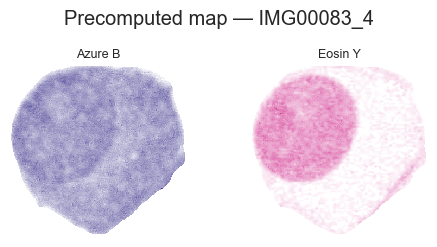
\includegraphics[width=0.5\textwidth]{figures/cell29.png}
    \caption{Precomputed concentration map for one cell, split into its two dye
    channels.}
    \label{fig:precomputed-map}
\end{figure}

\subsection{Training the Generative Model}
\label{subsec:train-diffusion}

A \textbf{diffusion model} (DDPM) is used to generate new plasma cells. It has
two directions:

\begin{itemize}
    \item \textbf{Forward} --- add Gaussian noise to a real concentration map,
          step by step, until it is pure noise.
    \item \textbf{Reverse} --- a \textbf{UNet} predicts the noise added at a
          given step; generation starts from pure noise and removes it step by
          step until a clean map remains.
\end{itemize}

Training uses the forward process as supervision: pick a random step, add that
much noise, and train the UNet to predict the noise, with an MSE loss between
predicted and true noise. The model trains on the concentration maps of
Section~\ref{subsec:color-deconvolution}, resized to $64\times64$ and normalized
with the dataset's per-channel mean and standard deviation. A usable model needs
many epochs on a GPU; pretrained weights are loaded for generation
(Section~\ref{subsec:generate-cells}).

\subsection{Generating Synthetic Cells}
\label{subsec:generate-cells}

Generation runs the \textbf{reverse diffusion}: starting from Gaussian noise,
noise is removed over the scheduler steps down to a clean 2-channel map, which
is then denormalized ($x \cdot \sigma + \mu$). To view a generated map as RGB,
the color deconvolution of Section~\ref{subsec:color-deconvolution} is inverted:

\begin{equation}
    I = I_0 \cdot 10^{-C \cdot S}
    \label{eq:inverse-beer-lambert}
\end{equation}

for a background light $I_0$. Figure~\ref{fig:generated-cells} shows generated
cells rendered on a near-white light, so that each cell can be inspected on a
pale field.

\begin{figure}[htbp]
    \centering
    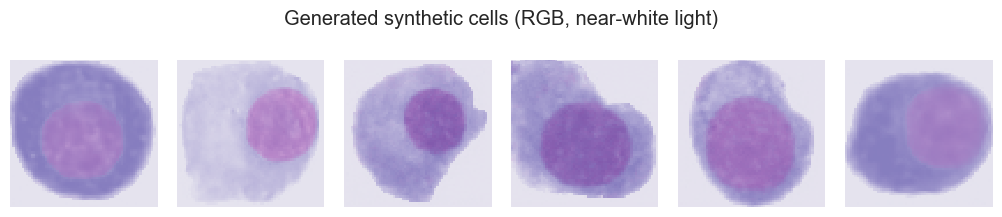
\includegraphics[width=\textwidth]{figures/cell35.png}
    \caption{Synthetic plasma cells sampled from the trained diffusion model,
    rendered in RGB under a near-white background light.}
    \label{fig:generated-cells}
\end{figure}

\subsection{Composing Full Synthetic Smears}
\label{subsec:compose-smears}

The two halves of the pipeline are combined: a \textbf{template}
(Section~\ref{subsec:kde-templates}) supplies a background color and
non-overlapping $(x, y, \text{size})$ boxes, and the \textbf{generative model}
(Section~\ref{subsec:generate-cells}) supplies one plasma cell per box. Each
generated concentration map is rebuilt as RGB via
Equation~\ref{eq:inverse-beer-lambert}, now using the \textbf{template's
background color} as $I_0$. Since the model's background is not exactly zero, a
raw square paste would leave a faint tinted box; instead, a \textbf{soft mask}
is built from the concentration (opaque on the cell, transparent near zero) and
used to paste each cell, so only the cell lands and the template background
shows elsewhere. Figure~\ref{fig:synthetic-smears} shows three full synthetic
smears produced this way.

\begin{figure}[htbp]
    \centering
    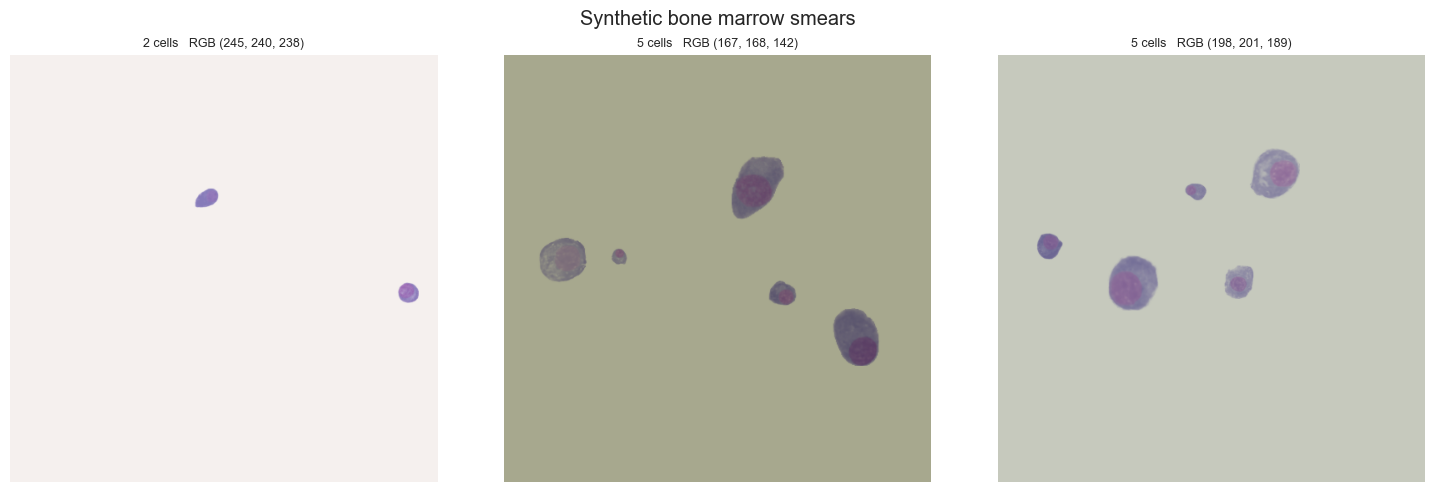
\includegraphics[width=\textwidth]{figures/cell37.png}
    \caption{Full synthetic bone marrow smears: generated plasma cells pasted
    onto KDE-sampled background templates through a soft concentration mask.}
    \label{fig:synthetic-smears}
\end{figure}

\subsection{Evaluation: Baseline vs. Augmented Detection}
\label{subsec:evaluation}

Two YOLO26-n detectors are compared: a \textbf{baseline}, trained only on the
real training set, and an \textbf{augmented} model, trained on the same data
plus 40\% DDPM-synthesized plasma cells from this pipeline. Both predict a
single class, \texttt{plasma\_cell}, at confidence 0.25.
Figure~\ref{fig:detection-comparison} overlays predictions (green, dashed) on
ground-truth boxes (red) for two test images where the augmented model fixes a
baseline failure:

\begin{itemize}
    \item \texttt{P\_20221113\_162935.jpg} --- the baseline emits four false
          positives; the augmented model returns the three true cells only.
    \item \texttt{P\_20221113\_165335.jpg} --- the baseline misses one of three
          cells; the augmented model detects all three, with no false positives
          in either case.
\end{itemize}

\begin{figure}[htbp]
    \centering
    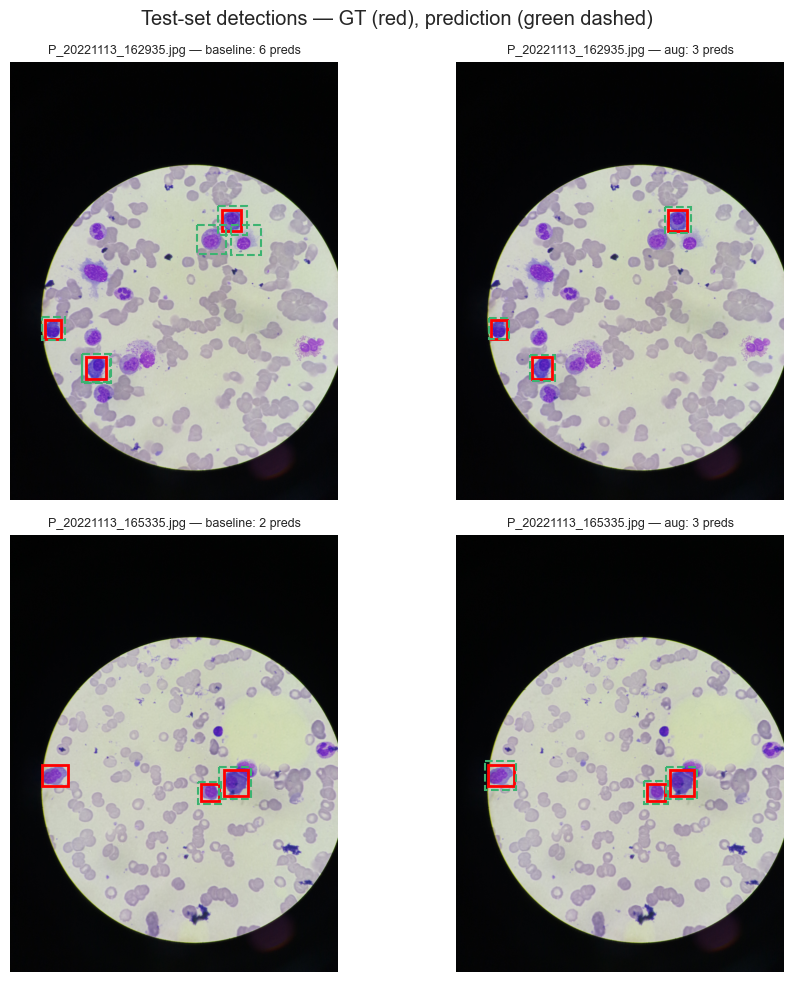
\includegraphics[width=0.85\textwidth]{figures/cell39.png}
    \caption{Baseline vs.\ augmented test-set detections on two held-out images.
    Ground truth in red, predictions in dashed green.}
    \label{fig:detection-comparison}
\end{figure}
